\newpage
\section{Registrazione}
Per poter usufruire delle funzionalità complete dell'API Market, quali acquisto e vendita di API, è necessario registrarsi. \MakeUppercase{è} possibile registrarsi alla piattaforma premendo il pulsante preposto nella barra superiore. La schermata che apparirà all'utente sarà la seguente:

\label{Registrazione}
\begin{figure}[H]
	\centering
	\fbox{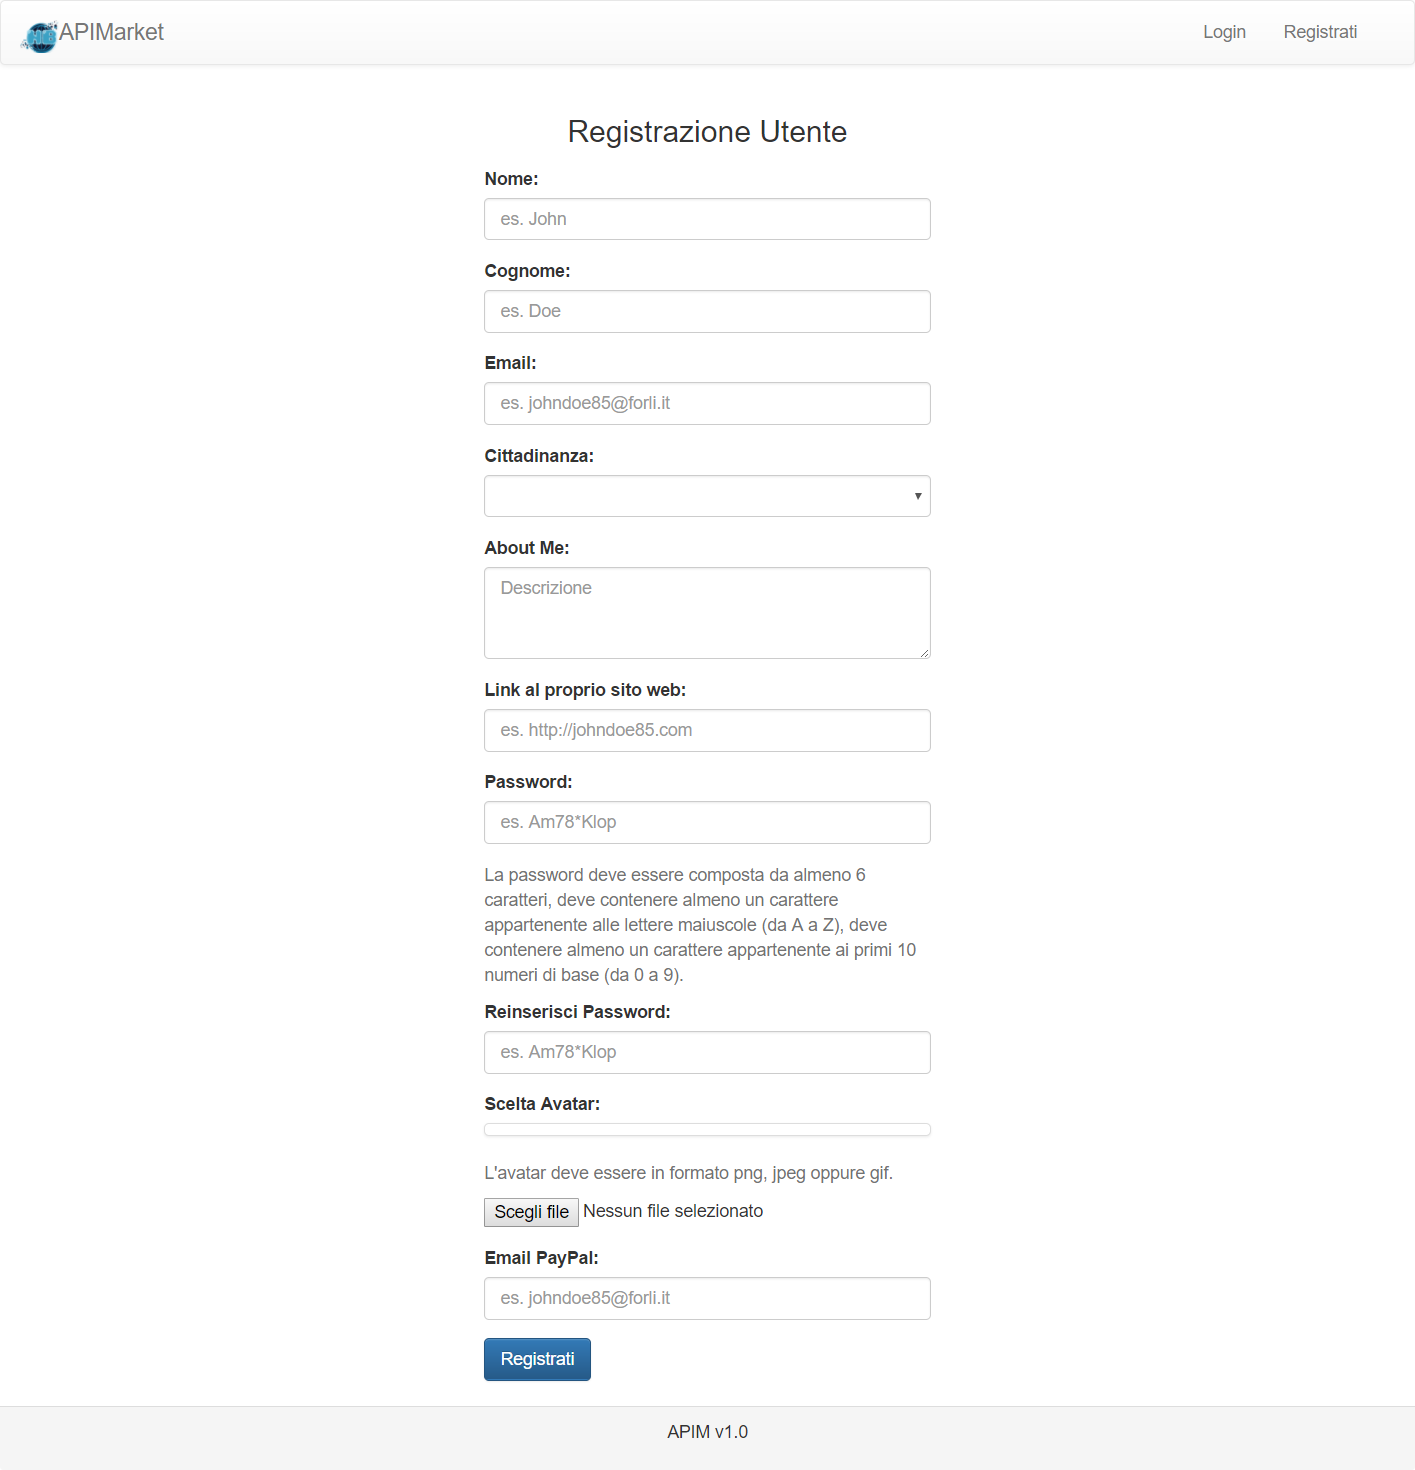
\includegraphics[scale=0.31]{img/APIM_registrazione.JPG}}
	\caption{Registrazione}
\end{figure}

un utente per registrasi dovrà compilare correttamente i seguenti campi, che sono obbligatori:
\begin{itemize}
	\item Nome;
	\item Cognome;
	\item Username desiderato;
	\item Stato di residenza;
	\item Indirizzo e-mail;
	\item Password desiderata;
	\item Conferma password.
\end{itemize}

Qualora questi dati non fossero presenti o corretti, il sistema segnala un errore all'atto di registrazione e l'utente deve inserire dei parametri validi nei campi indicati. Sono presenti inoltre dei campi opzionali:

\begin{itemize}
	\item Descrizione personale;
	\item Immagine personale;
	\item Email PayPal.
\end{itemize}

Questi campi, seppur non obbligatori, bloccano la registrazione qualora il loro inserimento non fosse effettuato in modo corretto. Si prega di prestare attenzione ai requisiti visualizzati nella schermata di registrazione.

\subsection{Login}

Tramite la barra superiore, vicino al pulsante di registrazione è possibile effettuare il login. La schermata di login può essere visualizzata a partire da ogni pagina non autenticata, selezionando l'apposita voce.
Il login può essere effettuato da un utente precedentemente registrato e dalla schermata di login è possibile autenticarsi nella piattaforma per poter svolgere le funzionalità preposte agli utenti registrati. 

\label{Login}
\begin{figure}[H]
	\centering
	\fbox{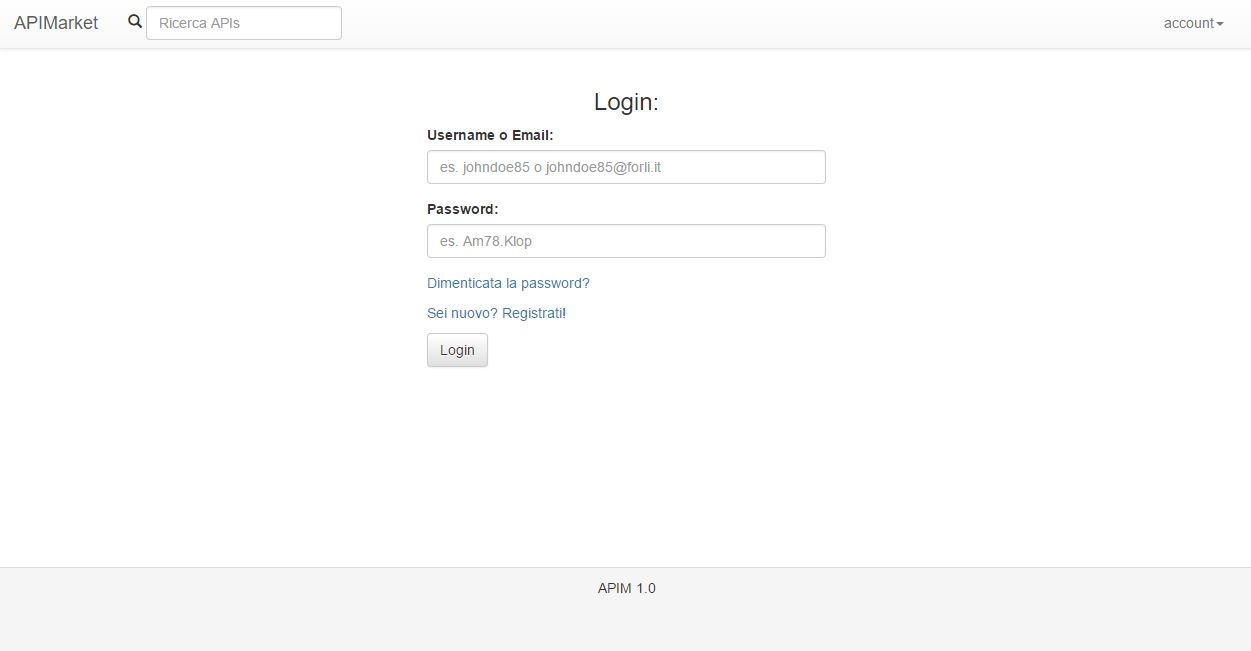
\includegraphics[scale=0.31]{img/APIM_login.JPG}}
	\caption{Login}
\end{figure}

\subsection{Conferma Login}
Dopo aver inserito i dati di login e cliccato sul pulsante "Login", se i dati di accesso sono corretti, l'utente visualizza una pagina di conferma login, con la possibilità di recarsi sulla Homepage oppure nella gestione del proprio profilo.

\label{Conferma Login}
\begin{figure}[H]
	\centering
	\fbox{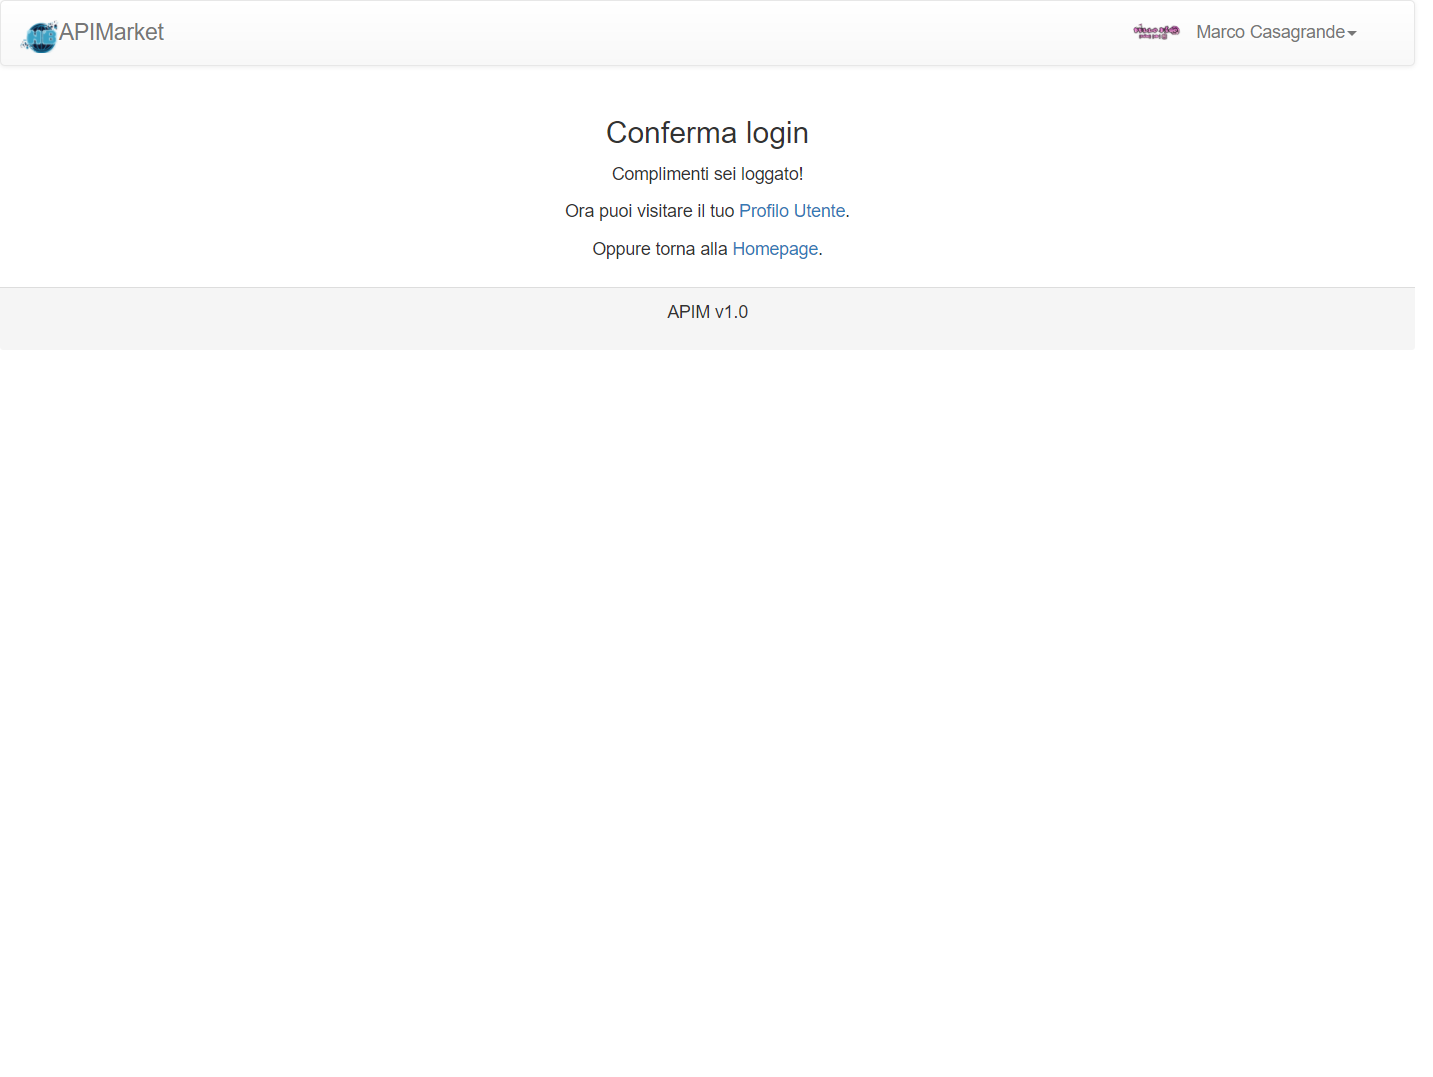
\includegraphics[scale=0.31]{img/APIM_confermaLogin.jpg}}
	\caption{Login}
\end{figure}



\subsection{Recupero Password}
Qualora si fosse dimenticata la password, dalla schermata di login si può accedere alla pagina per il recupero della password. Inserendo l'indirizzo email si può ottenere un link per reimpostare i propri dati personali tramite una pagina dedicata. 

\label{Recupero Password}
\begin{figure}[H]
	\centering
	\fbox{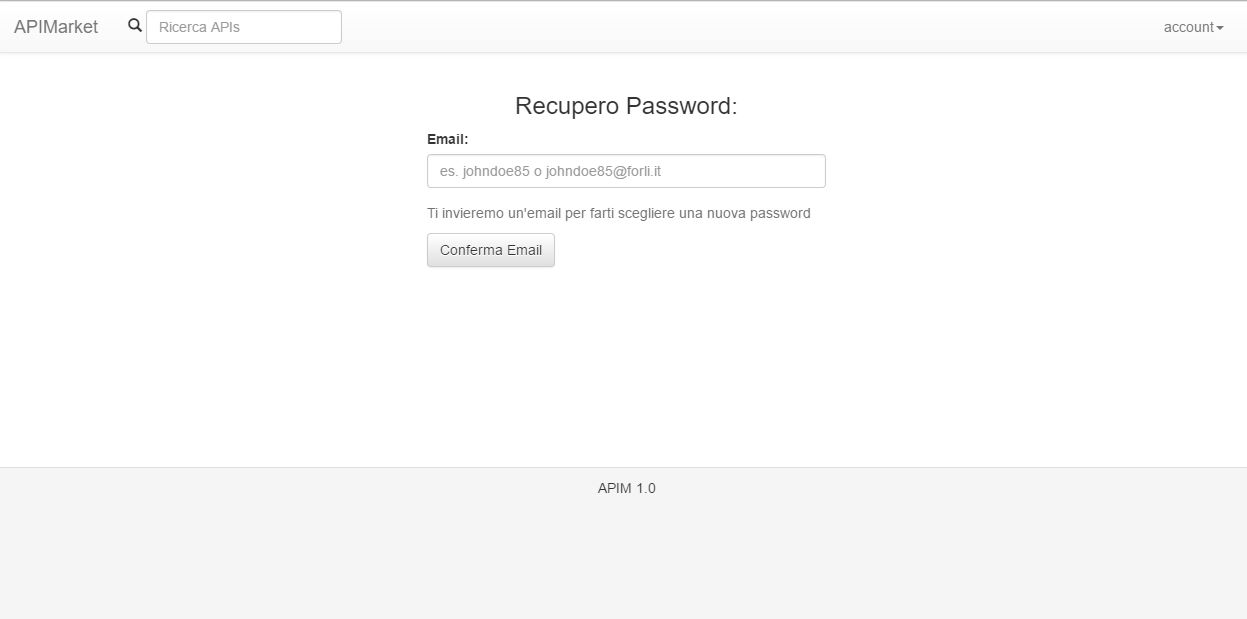
\includegraphics[scale=0.31]{img/APIM_recuperoPSW.JPG}}
	\caption{Recupero Password}
\end{figure}
